\section{Worked example}
\label{app:example}

This appendix applies the complete procedure to the canonical scenario of
\cref{sec:scope-scenario}. Both drivers are named models, and every
parameter used is taken from a public manufacturer datasheet. The
accompanying data manifest records the exact source URLs and SI input
records; \cref{tab:worked-pair} summarizes the computed results and is the
authoritative source where a number below is rounded.

\subsection*{Selected system}

\textbf{Low-bass manifold.} Two Dayton Audio UMII18-22 units arranged as
one mechanically opposed pair, permitting first-order reaction-force
cancellation under matched drive and mounting. Driver mismatch and
mounting tolerances leave residual force. The suffix ``22'' denotes dual
\SI{2}{\ohm} voice coils; the manufacturer's one-way linear excursion is
\SI{28}{\milli\meter}. The two drivers carry one common mono signal and share the
manifold target of \SI{110}{dB} \emph{in total} at
$r_{\mathrm{listen}}=\SI{3}{\meter}$ (basis B3); each has its own amplifier
channel. The $4\Vas$ cap binds at \SI{993}{\liter} per driver, giving
$\Qtc\simeq0.592$ and $F_c\simeq\SI{24.6}{\hertz}$. The resulting
\SI{1.99}{\cubic\meter} total enclosure is retained as a visible packaging
cost rather than hidden by a role-wide cap.

\textbf{Upper bass.} One FaitalPRO 12HP1030 per independent stereo
channel in \SI{16.6}{\liter}, giving $\Qtc\simeq0.539$ and
$F_c\simeq\SI{80}{\hertz}$, exactly at the split. Each channel meets its
own \SI{105}{dB} target at \SI{3}{\meter} (basis B4) with no credit from
the opposite channel. Publication calculations use the current official
manufacturer record, including $\Sd=\SI{518}{\centi\meter\squared}$,
$\Vas=\SI{35.9}{\liter}$ and
$\Xmax=\SI{12.45}{\milli\meter}$.

\subsection*{Demand and gates}

With $V_{\mathrm{room}}=\SI{60}{\cubic\meter}$ and
$L_{\max}=\SI{6}{\meter}$, $f_{\mathrm{pz}}\simeq\SI{28.6}{\hertz}$. Under
the declared \SI{10}{\hertz} leakage corner the worst low-bass demand
occurs at the bottom of the band, \SI{15}{\hertz}, and equals
\SI{4.57}{\liter} of peak displaced volume for the manifold as a whole
(\cref{tab:room-sensitivity}), hence about \SI{2.29}{\liter} per driver.

The realized alignment differs from the preferred $\Qtc^\ast=0.55$ because
the box cap binds. Its finite-band correction is not assumed free: any
boost is charged to \cref{eq:Preq,eq:Ereq,eq:Ireq}, excursion and burst
response, and the resulting worst-case values are checked against the
gates.
Across the complete \SIrange{15}{80}{\hertz} band the low-bass units run at
approximately $\xi_x\simeq0.689$ steady and
$\xi_x^{\mathrm{tr}}\simeq0.795$ for the declared one-cycle burst family.
The largest amplifier-budget utilization is about 0.642, inside the
\SI{90}{\volt}, \SI{15}{\ampere}, \SI{500}{\watt} continuous and
\SI{1}{\kilo\watt} burst limits and the driver's own rating.

The upper-bass channel uses $\xi_x\simeq0.485$ steady and
$\xi_x^{\mathrm{tr}}\simeq0.557$; its Doppler first-sideband ratio is
0.0138 and its largest amplifier-budget utilization is about 0.597.
Both roles are inside the hard $\Xmax$ boundary and the 0.80 preferred
excursion margin.
\Cref{fig:worked-system}
collects the separately reported indicators for both roles, and
\cref{fig:output-electrical} shows the corresponding output margin and
electrical utilization across each role's band.

\begin{figure}[htbp]
	\centering
	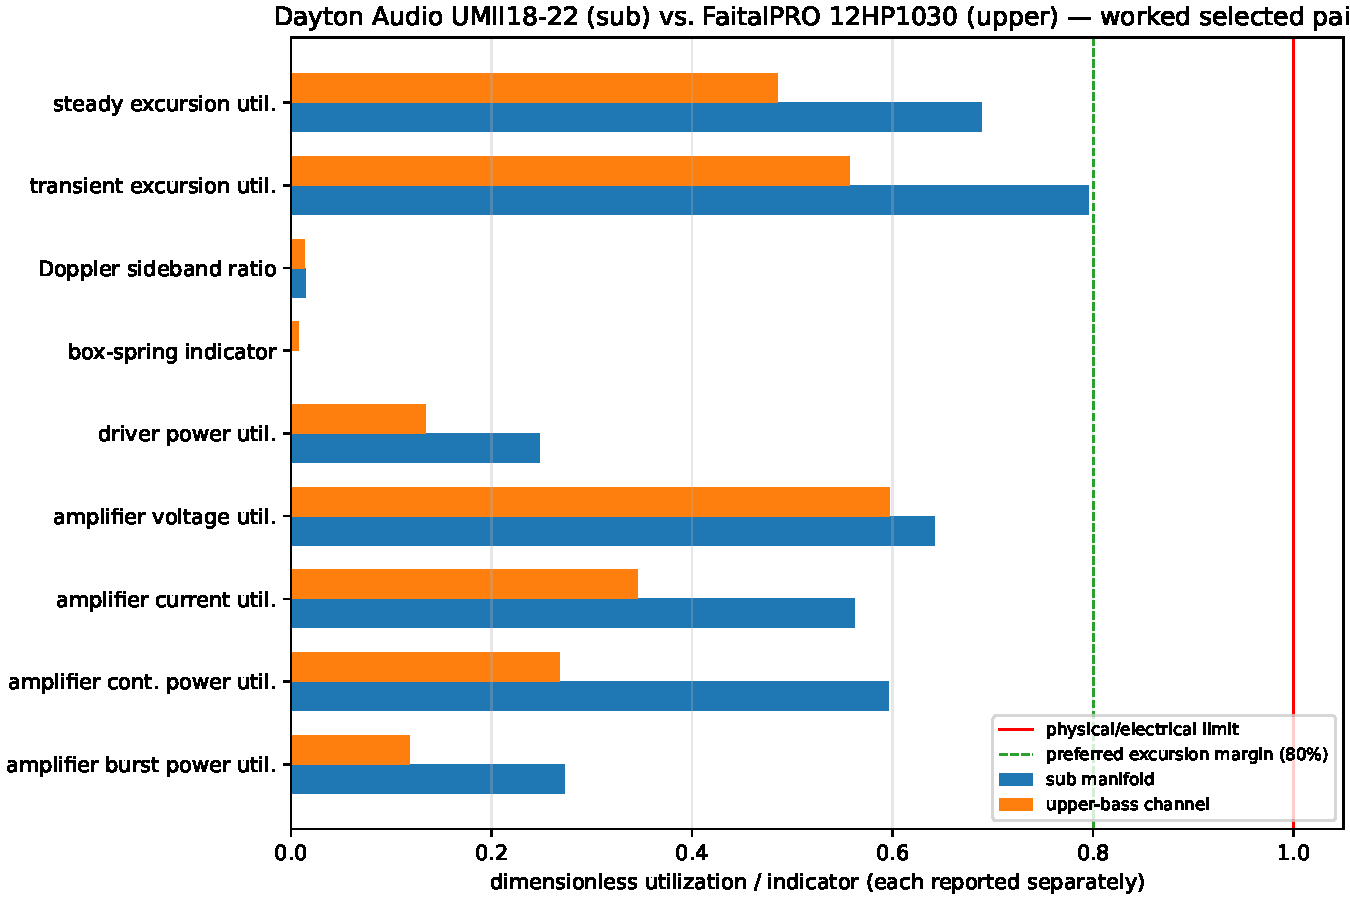
\includegraphics[width=\columnwidth]{../figures/fig_worked_system}
	\caption{Complete worked system: the dimensionless indicators of
	\cref{eq:riskvec} for the mono low-bass manifold and for one independent
	stereo upper-bass channel, against the hard limit and the preferred
	excursion margin. Each indicator is reported separately; none is summed
	with another.}
	\label{fig:worked-system}
\end{figure}

\begin{table*}[htbp]
\centering
\caption{Worked selected pair: Dayton Audio UMII18-22 (mono sub manifold, 2 identical units in an even, symmetrically opposed pairing -- permitting first-order reaction-force cancellation under matched drive and mounting; the even count is a hard mechanical-layout constraint, not a ranking-policy preference -- each with its own amplifier channel, aggregate target 110 dB for the manifold, not per driver) and FaitalPRO 12HP1030 (upper-bass, one unit per independent stereo channel, target 105 dB per channel). Pareto front number is one-based and is against this report's frozen private-database candidate pool for each role.}
\label{tab:worked-pair}
\small
\begin{tabular}{p{4.0cm}p{5.1cm}p{5.1cm}}
\toprule
 & Dayton UMII18-22 (sub) & FaitalPRO 12HP1030 (upper)\\
\midrule
public source & Dayton Audio official UMII18-22 specification sheet & FaitalPRO official 12HP1030 product data (8 ohm)\\
role, units & mono sub manifold, 2x (even, opposed pairs for first-order force cancellation when matched), aggregate target 110 dB for the manifold & stereo upper-bass, 1x per channel, target 105 dB per channel\\
$V_d$ per driver [L] & 3.32 & 0.64\\
$\eta_0 P_{\max}$ [W$_{\mathrm{ac}}$] & 4.63 & 10.32\\
$F_s$ / $Q_{ts}$ & 22 Hz / 0.530 & 45 Hz / 0.303\\
$f_L=\Re/2\pi\Le$ [Hz] & 581 & 589\\
box per driver: $V_b$, $F_c$ & 993 L, 24.6 Hz & 16.6 L, 80.0 Hz\\
$Q_{tc}$ & 0.592 & 0.539\\
worst steady excursion util. & 0.69 & 0.48\\
worst transient excursion util. & 0.80 & 0.56\\
worst voltage [V rms @ Hz] & 56.9 @ 28.6 & 53.7 @ 80.0\\
worst current [A rms @ Hz] & 8.4 @ 80.0 & 5.2 @ 250.0\\
worst power [W @ Hz] & 298 @ 80.0 & 134 @ 250.0\\
Pareto front / status & 1 / feasible & 1 / feasible\\
\bottomrule
\end{tabular}
\end{table*}


\subsection*{Reading the result}

Three points matter more than the specific models.

First, the binding trade differs by role. For the low-bass manifold the
$4\Vas$ cap fixes a very large enclosure and its correction demand; for the
upper-bass channel the crossover controls excursion and Doppler margin.
Neither is visible from an output-ceiling comparison alone.

Second, the two roles are served by candidates from different regions of
the descriptor plane (\cref{fig:database-pareto}). Within this candidate
population and scenario, the alternatives that rank close to each selection
do so for role-specific reasons---greater $\Vd$ at higher electrical demand
for the low-bass role, greater $\eta_0\Pmax$ at lower $f_L$ for the
upper-bass role---and their Pareto and policy statuses are reported in
\cref{tab:worked-pair} rather than reduced to a single score.

The earlier hard-$\Qtc$/role-volume formulation selected a costly
high-flux professional 18-inch driver largely because it excluded
high-$\Qts$, high-stroke alternatives geometrically. Under the revised
policy the UMII18-22 pays explicitly for its box and equalization, yet
remains Pareto-optimal. The selected model is therefore a consequence of
the declared physical and electronics tradeoffs, not of treating
$F_s< f_{\mathrm{pz}}$ or $\Qtc\le0.55$ as mandatory.

Third, the result is conditional on the room. \Cref{tab:room-sensitivity}
shows how the required displaced volume, and hence the driver count, moves
with the assumed leakage corner; a less favourable corner is absorbed here
by the manifold's excursion margin, but that margin is finite and is
reported rather than assumed.
